\documentclass{ximera}

\usepackage{epsfig}

\graphicspath{
  {./}
  {figures/}
}

\usepackage{epstopdf}
%\usepackage{ulem}
\usepackage[normalem]{ulem}

\epstopdfsetup{outdir=./}

\usepackage{morewrites}
\makeatletter
\newcommand\subfile[1]{%
\renewcommand{\input}[1]{}%
\begingroup\skip@preamble\otherinput{#1}\endgroup\par\vspace{\topsep}
\let\input\otherinput}
\makeatother

\newcommand{\EXER}{}
\newcommand{\includeexercises}{\EXER\directlua{dofile(kpse.find_file("exercises","lua"))}}

\newenvironment{computerExercise}{\begin{exercise}}{\end{exercise}}

%\newcounter{ccounter}
%\setcounter{ccounter}{1}
%\newcommand{\Chapter}[1]{\setcounter{chapter}{\arabic{ccounter}}\chapter{#1}\addtocounter{ccounter}{1}}

%\newcommand{\section}[1]{\section{#1}\setcounter{thm}{0}\setcounter{equation}{0}}

%\renewcommand{\theequation}{\arabic{chapter}.\arabic{section}.\arabic{equation}}
%\renewcommand{\thefigure}{\arabic{chapter}.\arabic{figure}}
%\renewcommand{\thetable}{\arabic{chapter}.\arabic{table}}

%\newcommand{\Sec}[2]{\section{#1}\markright{\arabic{ccounter}.\arabic{section}.#2}\setcounter{equation}{0}\setcounter{thm}{0}\setcounter{figure}{0}}
  
\newcommand{\Sec}[2]{\section{#1}}

\setcounter{secnumdepth}{2}
%\setcounter{secnumdepth}{1} 

%\newcounter{THM}
%\renewcommand{\theTHM}{\arabic{chapter}.\arabic{section}}

\newcommand{\trademark}{{R\!\!\!\!\!\bigcirc}}
%\newtheorem{exercise}{}

\newcommand{\dfield}{{\sf SlopeField}}

\newcommand{\pplane}{{\sf PhasePlane}}

\newcommand{\PPLANE}{{\sf PHASEPLANE}}

% BADBAD: \newcommand{\Bbb}{\bf}. % Package amsfonts Warning: Obsolete command \Bbb; \mathbb should be used instead.

\newcommand{\R}{\mbox{$\mathbb{R}$}}
\let\C\relax
\newcommand{\C}{\mbox{$\mathbb{C}$}}
\newcommand{\Z}{\mbox{$\mathbb{Z}$}}
\newcommand{\N}{\mbox{$\mathbb{N}$}}
\newcommand{\D}{\mbox{{\bf D}}}

\newcommand{\WW}{\mathcal{W}}

\usepackage{amssymb}
%\newcommand{\qed}{\hfill\mbox{\raggedright$\square$} \vspace{1ex}}
%\newcommand{\proof}{\noindent {\bf Proof:} \hspace{0.1in}}

\newcommand{\setmin}{\;\mbox{--}\;}
\newcommand{\Matlab}{{M\small{AT\-LAB}} }
\newcommand{\Matlabp}{{M\small{AT\-LAB}}}
\newcommand{\computer}{\Matlab Instructions}
\renewcommand{\computer}{M\small{ATLAB} Instructions}
\newcommand{\half}{\mbox{$\frac{1}{2}$}}
\newcommand{\compose}{\raisebox{.15ex}{\mbox{{\scriptsize$\circ$}}}}
\newcommand{\AND}{\quad\mbox{and}\quad}
\newcommand{\vect}[2]{\left(\begin{array}{c} #1_1 \\ \vdots \\
 #1_{#2}\end{array}\right)}
\newcommand{\mattwo}[4]{\left(\begin{array}{rr} #1 & #2\\ #3
&#4\end{array}\right)}
\newcommand{\mattwoc}[4]{\left(\begin{array}{cc} #1 & #2\\ #3
&#4\end{array}\right)}
\newcommand{\vectwo}[2]{\left(\begin{array}{r} #1 \\ #2\end{array}\right)}
\newcommand{\vectwoc}[2]{\left(\begin{array}{c} #1 \\ #2\end{array}\right)}

\newcommand{\ignore}[1]{}


\newcommand{\inv}{^{-1}}
\newcommand{\CC}{{\cal C}}
\newcommand{\CCone}{\CC^1}
\newcommand{\Span}{{\rm span}}
\newcommand{\rank}{{\rm rank}}
\newcommand{\trace}{{\rm tr}}
\newcommand{\RE}{{\rm Re}}
\newcommand{\IM}{{\rm Im}}
\newcommand{\nulls}{{\rm null\;space}}

\newcommand{\dps}{\displaystyle}
\newcommand{\arraystart}{\renewcommand{\arraystretch}{1.8}}
\newcommand{\arrayfinish}{\renewcommand{\arraystretch}{1.2}}
\newcommand{\Start}[1]{\vspace{0.08in}\noindent {\bf Section~\ref{#1}}}
\newcommand{\exer}[1]{\noindent {\bf \ref{#1}}}
\newcommand{\ans}{\textbf{Answer:} }
\newcommand{\matthree}[9]{\left(\begin{array}{rrr} #1 & #2 & #3 \\ #4 & #5 & #6
\\ #7 & #8 & #9\end{array}\right)}
\newcommand{\cvectwo}[2]{\left(\begin{array}{c} #1 \\ #2\end{array}\right)}
\newcommand{\cmatthree}[9]{\left(\begin{array}{ccc} #1 & #2 & #3 \\ #4 & #5 &
#6 \\ #7 & #8 & #9\end{array}\right)}
\newcommand{\vecthree}[3]{\left(\begin{array}{r} #1 \\ #2 \\
#3\end{array}\right)}
\newcommand{\cvecthree}[3]{\left(\begin{array}{c} #1 \\ #2 \\
#3\end{array}\right)}
\newcommand{\cmattwo}[4]{\left(\begin{array}{cc} #1 & #2\\ #3
&#4\end{array}\right)}

\newcommand{\Matrix}[1]{\ensuremath{\left(\begin{array}{rrrrrrrrrrrrrrrrrr} #1 \end{array}\right)}}

\newcommand{\Matrixc}[1]{\ensuremath{\left(\begin{array}{cccccccccccc} #1 \end{array}\right)}}



\renewcommand{\labelenumi}{\theenumi}
\newenvironment{enumeratea}%
{\begingroup
 \renewcommand{\theenumi}{\alph{enumi}}
 \renewcommand{\labelenumi}{(\theenumi)}
 \begin{enumerate}}
 {\end{enumerate}
 \endgroup}

\newcounter{help}
\renewcommand{\thehelp}{\thesection.\arabic{equation}}

%\newenvironment{equation*}%
%{\renewcommand\endequation{\eqno (\theequation)* $$}%
%   \begin{equation}}%
%   {\end{equation}\renewcommand\endequation{\eqno \@eqnnum
%$$\global\@ignoretrue}}

%\input{psfig.tex}

\author{Martin Golubitsky and Michael Dellnitz}

%\newenvironment{matlabEquation}%
%{\renewcommand\endequation{\eqno (\theequation*) $$}%
%   \begin{equation}}%
%   {\end{equation}\renewcommand\endequation{\eqno \@eqnnum
% $$\global\@ignoretrue}}

\newcommand{\soln}{\textbf{Solution:} }
\newcommand{\exercap}[1]{\centerline{Figure~\ref{#1}}}
\newcommand{\exercaptwo}[1]{\centerline{Figure~\ref{#1}a\hspace{2.1in}
Figure~\ref{#1}b}}
\newcommand{\exercapthree}[1]{\centerline{Figure~\ref{#1}a\hspace{1.2in}
Figure~\ref{#1}b\hspace{1.2in}Figure~\ref{#1}c}}
\newcommand{\para}{\hspace{0.4in}}

\usepackage{ifluatex}
\ifluatex
\ifcsname displaysolutions\endcsname%
\else
\renewenvironment{solution}{\suppress}{\endsuppress}
\fi
\else
\renewenvironment{solution}{}{}
\fi

\ifcsname answer\endcsname
\renewcommand{\answer}{}
\fi

%\ifxake
%\newenvironment{matlabEquation}{\begin{equation}}{\end{equation}}
%\else
\newenvironment{matlabEquation}%
{\let\oldtheequation\theequation\renewcommand{\theequation}{\oldtheequation*}\begin{equation}}%
  {\end{equation}\let\theequation\oldtheequation}
%\fi

\makeatother

\newcommand{\RED}[1]{{\color{red}{#1}}} 


\title{Preface}

\begin{document}
\begin{abstract}
\end{abstract}
\maketitle

%\section*{Preface}

These notes provide an integrated approach to linear algebra and ordinary 
differential equations based on computers --- in this case the software 
package \Matlabp$^\trademark$ \footnote{\Matlab is a registered trademark
of The MathWorks Inc. Natick, MA}.   We believe that computers can improve 
the conceptual understanding of mathematics --- not just enable the 
completion of complicated calculations.  We use computers in two ways:  in 
linear algebra computers reduce the drudgery of calculations and 
enable students to focus on concepts and methods, while in differential 
equations computers display phase portraits graphically and enable 
students to focus on the qualitative information embodied in solutions 
rather than just on developing formulas for solutions.

We develop methods for solving both systems of linear 
equations and systems of (constant coefficient) linear ordinary 
differential equations.  It is generally accepted that linear algebra 
methods aid in finding closed form solutions to systems of linear 
differential equations.  The fact that the graphical solution of systems 
of differential equations can motivate concepts (both geometric and algebraic)
in linear algebra is less often discussed.  These notes begin by solving linear 
systems of equations (through standard Gaussian elimination theory) and 
discussing elementary matrix theory.  We then introduce simple differential 
equations --- both single equations and planar systems --- to motivate the 
notions of eigenvectors and eigenvalues. In subsequent chapters linear algebra 
and ODE theory are often mixed.  

Regarding differential equations, our purpose is to introduce at the 
sophomore -- junior level ideas from dynamical systems theory.  We focus on 
phase portraits (and time series) rather than on techniques for finding
closed form solutions.  We assume that now and in the future practicing
scientists and mathematicians will use ODE solving computer programs
more frequently than they will use techniques of integration.  For this
reason we have focused on the information that is embedded in the computer  
graphical approach.  We discuss both typical phase portraits
(Morse-Smale systems) and typical one parameter bifurcations (both local 
and global).   Our goal is to provide the mathematical background that is
needed when interpreting the results of computer simulation.

\paragraph{The integration of computers:}  Our approach assumes that students 
have an easier time learning with 
computers if the computer segments are fully integrated with the course 
material.  So we have interleaved the instructions on how to use \Matlab 
with the examples and theory in the text.  With ease of use in mind, we 
have also provided a number of preloaded matrices and differential equations 
with the notes.  Any equation label in this text that is followed by an 
asterisk can be loaded into \Matlab just by typing the formula number.  For 
the successful use of this text, it is important that students have access 
to computers with \Matlab and the computer files associated with these notes.

John Polking developed an excellent graphical user interface for solving
planar systems of autonomous differential equations called {\textsf{pplane}}.  
This program has been updated by Roy Goodman and is now called {\pplane}.
%Until Chapter~\ref{C:HDS}
We use {\pplane} instead of using the \Matlab native commands for solving ODEs. 
In these notes we also provide an introduction to {\pplane}. 
%and the other associated software routines.

For the most part we treat the computer as a black box.  We have not
attempted to explain how the computer, or more precisely \Matlabp, 
performs computations.   Linear algebra structures are developed (typically) 
with proofs, while differential equations theorems are presented (typically) 
without proof and are instead motivated by computer experimentation.  

There are two types of exercises included with most sections --- those that 
should be completed using pencil and paper (called Hand Exercises) and 
those that should be completed with the assistance of computers (called 
Computer Exercises).  

\paragraph{Ways to use the text:}  We envision this course as a one-year 
sequence replacing the standard one semester linear algebra and ODE courses. 
There is a natural one semester {\em Linear Systems\/} course that can be 
taught using the material in this book. In this course students will
learn both the basics of linear algebra and the basics of linear systems of
differential equations.  This one semester course covers the material in the 
first eight chapters.  The {\em Linear Systems\/} course stresses eigenvalues 
and a baby Jordan normal form theory for $2\times 2$ matrices and culminates 
in a classification of phase portraits for planar constant coefficient linear 
systems of differential equations.   Time permitting additional linear 
algebra topics from Chapters~9 and 10 may be included.  Such material 
includes changes of coordinates for linear mappings, and orthogonality 
including Gram-Schmidt orthonormalization and least squares fitting of data.

We believe that by being exposed to ODE theory a student taking just the 
first semester of this sequence will gain a better appreciation of linear 
algebra than will a student who takes a standard one semester introduction 
to linear algebra.  However, a more traditional {\em Linear Algebra\/} course 
can be taught by omitting Chapter 7 and de-emphasizing some of the material 
in Chapter 6.  Then there will be time in a one semester course to cover a 
selection of the linear algebra topics mentioned at the end of the previous 
paragraph. 

%A schematic diagram of the dependency relations between chapters is given in
%Figure~\ref{F:depdiag}.  Note that if two arrows in that figure point towards 
%the same chapter, then material in both of the preceding chapters will be 
%needed to complete the given chapter.  Of particular importance is the
%observation that the material in Chapter \ref{Chap:LinTrans}
% , \ref{C:BT}, and \ref{ch:NumSolODE}
%may be omitted without repercussion.

%\begin{figure}[htb]
%     \centerline{%
%     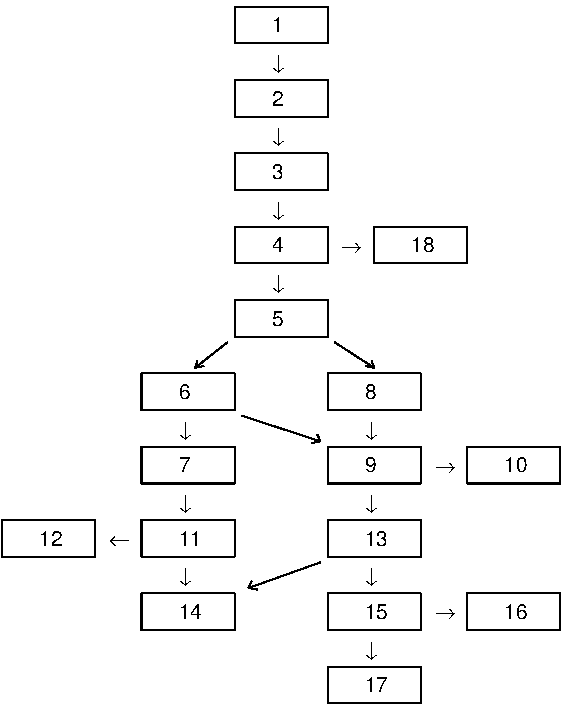
\includegraphics{figures/depdiag.pdf}}
%     \caption{Dependency relations between chapters.}
%     \label{F:depdiag}
%\end{figure}

%\subsection*{Comments on Individual Chapters}

\paragraph{Chapters~\ref{chap:prelim}--\ref{chap:matrices}}  We consider the 
first two chapters to be introductory material and we attempt to cover this 
material as quickly as we can.  Chapter~\ref{chap:prelim} introduces \Matlab 
along with elementary remarks on vectors and matrices.  In our course we ask 
the students to read the material in 
Chapter~\ref{chap:prelim} and to use the computer instructions in that
chapter as an entry into \Matlabp.  In class we cover only the material on
dot product.  Chapter~\ref{lineq} explains how to solve systems of linear
equations and is required for a first course on linear algebra.  The proof of
the uniqueness of reduced echelon form matrices is not very illuminating
for students and can be omitted in classroom discussion.  Sections whose
material we feel can be omitted are noted by asterisks in the Table of 
Contents and Section~\ref{S:uniquerowechelon} is the first example of such 
a section.

In Chapter~\ref{chap:matrices} we introduce matrix multiplication as a
notation that simplifies the presentation of systems of linear equations.
We then show how matrix multiplication leads to linear mappings and how    
linearity leads to the principle of superposition.  Multiplication of 
matrices is introduced as composition of linear mappings, which makes 
transparent the observation that multiplication of matrices is associative.  
The chapter ends with a discussion of inverse matrices and the role that
inverses play in solving systems of linear equations.  The determinant of 
a $2\times 2$ matrix is introduced and its role in determining matrix
inverses is emphasized. 

\paragraph{Chapter~\ref{chap:SolveOdes}} This chapter provides a nonstandard 
introduction to differential equations.  We begin by emphasizing that 
solutions to differential equations are functions (or pairs of functions for 
planar systems).  We explain in detail the two ways that we may graph 
solutions to differential equations (time series and phase space) and how to 
go back and forth between these two graphical representations.  The use of 
the computer is mandatory in this chapter.  Chapter~\ref{chap:SolveOdes} 
dwells on the qualitative theory of solutions to autonomous ordinary 
differential equations.  In one dimension we discuss the importance of 
knowing equilibria and their stability so that we can understand the fate of 
all solutions.  In two dimensions we emphasize constant coefficient linear 
systems and the existence (numerical) of invariant directions 
(eigendirections).  In this way we motivate the introduction of eigenvalues 
and eigenvectors, which are discussed in detail for $2\times 2$ matrices.  
Once we know how to compute eigenvalues and eigendirections, we then show how
this information coupled with superposition leads to closed form solution to
initial value problems, at least when the eigenvalues are real and distinct.

We are not trying 
to give a thorough grounding in techniques for solving differential equations 
in Chapter~\ref{chap:SolveOdes}; rather we are trying to give an introduction 
to the ways that modern computer programs will represent graphically 
solutions to differential equations.  We have included, however, a section on 
separation of variables for those who wish to introduce techniques for 
finding closed form solutions to single differential equations at this time.  
Our preference is to omit this section in the {\em Linear Systems\/} course 
as well as to omit the applications in Section~\ref{S:growthmodels} of the 
linear growth model in one dimension to interest rates and population 
dynamics.  

\paragraph{Chapter~\ref{C:vectorspaces}} In this chapter we introduce vector 
space theory: vector spaces, subspaces, spanning sets, linear independence, 
bases, dimensions and the other basic notions in linear algebra.  Since 
solutions to differential equations naturally reside in function spaces, we 
are able to illustrate that vector spaces other than $\R^n$ arise naturally.  
We have found that, depending on time, the proof of the main theorem, which 
appears in Section~\ref{S:5.6}, may be omitted in a first course.  The 
material in these chapters is mandatory in any first course on linear algebra.

%\paragraph{Chapters~\ref{Chap:Planar} and \ref{Chap:PlanarQ}}%, \ref{C:NPS}, and 
% \ref{C:BT}}

\paragraph{Chapter~\ref{Chap:Planar}}

At this juncture the text divides into two tracks: one concerned with
the qualitative theory of solutions to linear and nonlinear planar
systems of differential equations and one mainly concerned with the
development of higher dimensional linear algebra.  We begin with a
description of the differential equations chapters.

Chapter~\ref{Chap:Planar} describes closed form solutions to planar
systems of constant coefficient linear differential equations in two
different ways: a direct method based on eigenvalues and eigenvectors
 and a related method based on
similarity of matrices.  Each method has its virtues and
vices.  Note that the Jordan normal form theorem for $2\times 2$
matrices is proved when discussing how to solve linear planar systems
using similarity of matrices.

%The qualitative description of phase portraits (saddles, sinks,
%sources, stability, centers, etc.) for planar linear systems is
%presented in Chapter~\ref{Chap:PlanarQ}.  This description depends
%crucially on the linear algebra of $2\times 2$ matrices developed in
%Chapters~\ref{chap:matrices} and \ref{Chap:Planar}.

% In Chapter~\ref{C:NPS} we discuss the fact that nonlinear equations behave 
% like their linear counterparts in a neighborhood of a hyperbolic equilibrium 
% and we verify this fact through computer experimentation.  Periodic solutions 
% to planar systems are introduced through the use of phase--amplitude 
% equations.  The chapter ends with a description of Morse-Smale nonlinear 
% autonomous differential equations.  

% The discussion of planar systems of differential equations ends in
% Chapter~\ref{C:BT} with a discussion of the typical bifurcations that one 
% may expect with the variation of one parameter.  These bifurcations include
% saddle-node bifurcations, which create a pair of equilibria, Hopf
% bifurcations, which create limit cycles, and global bifurcations.  The
% discussion is framed around the breakdown of the linearization theorem at
% nonhyperbolic equilibria and the use of computer experimentation.  

% It is unusual to include the material in Chapters~\ref{C:NPS} and \ref{C:BT}
% in courses at this level.  We contend, however, that the material is
% accessible to students who feel comfortable with computer experimentation and
% provides an alternative to learning only techniques for finding closed form 
% solutions in a first course on differential equations.  Both approaches
% are important; but we believe that the geometric approach based on computer
% simulation will be more the norm in the future than will be the determination
% of closed form solutions.  Accordingly, we have arranged the material with
% the geometric theory appearing first and the techniques for finding closed
% form solutions appearing later.

\paragraph{Chapters~\ref{C:D&E}, \ref{C:LMCC}, \ref{Chap:LinTrans}, and 
  \ref{C:HDeigenvalues}}
%Material from these four chapters on linear algebra can be covered directly after Chapter~\ref{Chap:Planar}.
Chapter~\ref{C:D&E} 
discusses determinants, characteristic polynomials, and eigenvalues for
$n\times n$ matrices.  Chapter~\ref{C:LMCC} presents more advanced
material on linear mappings including row rank equals column rank and the
matrix representation of mappings in different coordinate systems.  The 
material in Sections~\ref{Sect:linmap} and \ref{S:5.8} could be presented 
directly after Chapter~\ref{C:vectorspaces}, while the material in
Section~\ref{S:coordinates} explains the geometric meaning of similarity.
%and requires the discussion of similar matrices in Chapter~\ref{Chap:Planar}.  

Orthogonal bases and orthogonal matrices, least squares and Gram-Schmidt
orthonormalization, and symmetric matrices are presented in 
Chapter~\ref{Chap:LinTrans}.  This material is very important, but is not 
required later in the text, and may be omitted.

The Jordan normal form theorem for $n\times n$ matrices is presented in 
Chapter~\ref{C:HDeigenvalues}.  Diagonalization of matrices with distinct
real and complex eigenvalues is presented in the first two sections.  The
appendices, including the proof of the complete Jordan normal form theorem,
are included for completeness and should be omitted in classroom
presentations.

% \paragraph{Chapter~\ref{C:HDS}}  In this chapter we present elements of the
% qualitative theory of autonomous systems of differential equations in higher
% dimensions.  A comprehensive discussion of this topic is far beyond a course 
% at this level.  We emphasize the $n$-dimensional version of linearization near
% an equilibrium (including asymptotic stability which uses the Jordan normal 
% form theorem of Chapter~\ref{C:HDeigenvalues}).  We also discuss some of the 
% complicated dynamics that appear in the solutions of systems of three and 
% four differential equations, including quasiperiodic motion (in linear and 
% nonlinear systems) and chaos (as represented by the Lorenz attractor).  In 
% order to explore these topics we need to introduce the \Matlab native routine 
% {\sf ode45} for solving systems of ordinary differential equations.

% \paragraph{Chapters~\ref{C:LDE}, \ref{C:LT}, \ref{chap:SingleOdes}, and 
% \ref{ch:NumSolODE}}  The material in the remaining chapters is material that 
% is more standard for a junior level course in ordinary differential equations.
% Chapter~\ref{C:LDE} discusses techniques for finding solutions of linear 
% systems and higher order linear equations.  This discussion requires 
% generalized eigenvectors and hence aspects of Jordan normal form.  We find 
% solutions to higher order equations by reducing them to first order systems.  
% Undetermined coefficients and resonance are also presented.  The popular 
% method of Laplace transforms 
% is discussed in Chapter~\ref{C:LT} and the importance of this method for
% solving forced linear equations (including discontinuous forcing) is
% emphasized.  The material on Laplace transforms could be presented after
% linearity has been discussed (after Chapter~\ref{C:vectorspaces} or even 
% after Chapter~\ref{chap:matrices}), but we do not recommend this approach.

% Chapter~\ref{chap:SingleOdes} discusses linear equations with nonconstant
% coefficients (variation of parameters and reduction of order) and several
% techniques (some elementary) for solving certain nonlinear equations.  These
% include substitution, exact differential equations, and planar Hamiltonian
% systems.

% The text ends with a discussion of numerical techniques in 
% Chapter~\ref{ch:NumSolODE}.  Euler and Runge-Kutta methods are presented. 
% This material could, in principle, be introduced as early as after
% Chapter~\ref{chap:SolveOdes}.   However, this material has been included more
% as an appendix than as an integrated part of the course.  These topics are
% appropriate as assignments for independent study by interested students.

\paragraph{The Classroom Use of Computers}  At the University of Houston we
use a classroom with an IBM compatible PC and an overhead display.  Lectures 
are presented three hours a week using a combination of blackboard and 
computer display.  We find it inadvisable to use the computer for more than 
five minutes at a time; we tend to go back and forth between standard lecture 
style and computer presentations.  (The preloaded matrices and differential 
equations are important to the smooth use of the computer in class.)  

We ask students to enroll in a one hour computer lab where they can practice 
using the material in the text on a computer, do their homework and additional
projects, and ask questions of TA's.  Our computer lab happens to have 15 
power macs.  In addition, we ensure that \Matlab and the {\sf laode} files are
available on student use computers around the campus (which is not always 
easy).  The {\sf laode} files are on the enclosed CDROM; they may also be 
downloaded by using a web browser or by anonymous ftp.
%See page ??? for instructions.

\paragraph{Acknowledgements} This course was first taught on a pilot
basis during the 1995--96 academic year at the University of Houston.
We thank the Mathematics Department and the College of Natural
Sciences and Mathematics of the University of Houston for providing
the resources needed to bring a course such as this to fruition.  We
gratefully acknowledge John Polking's help in adapting his software
for our use and for allowing us access to his code so that we could
write companion software for use in linear algebra.

We thank Denny Brown for his advice and his careful readings of the
many drafts of this manuscript.  We thank Gerhard Dangelmayr, Michael
Field, Michael Friedberg, Steven Fuchs, Kimber Gross, Barbara Keyfitz,
Charles Peters and David Wagner for their advice on the presentation
of the material.  We also thank Elizabeth Golubitsky, who has written
the companion {\em Solutions Manual\/}, for her help in keeping the
material accessible and in a proper order.  Finally, we thank the
students who stayed with this course on an experimental basis and by
doing so helped to shape its form.

\vspace{0.1in}

\noindent Houston and Bayreuth \hfill Martin Golubitsky \\
May, 1998  \hfill Michael Dellnitz




Columbus \hfill Martin Golubitsky  \\
February, 2018 \hfill James Fowler
\end{document}
